\PID \mnImportant \label{z:ct_stab}
Испитати асимптотску стабилност система који су дефинисани датом диференцијалном једначином у операторском облику
\begin{multicols}{2}
    \begin{enumerate}[label=(\alph*)]
    \item $(\DD + 1)^2(\DD + 2)y(t) = x(t)$;
    \item $(\DD^2 + 4)y(t) = x(t)$;
    \item $(\DD^2 + 9)^2 y(t) = x(t)$;
    \item $(\DD^2 - 4\DD + 5) y(t) = x(t)$.
    \end{enumerate}
\end{multicols} \noindent

\RESENJE
Асимтпторска стабилност зависи од могућих понашања одзива система услед његовог унутрашњег стања које је одређено почетним условима, односно, 
зависи од његовог сопственог одзива. Уколико сопствени одзив система тежи нули након довољно дуго времена, без обзира на почетне услове, 
за такав систем кажемо да је \textit{асимптотски стабилан}. Уколико сопствени одзив система тежи бесконачности, за неке почетне услове, онда кажемо 
да је он \textit{асимптотски нестабилан}. Уколико систем није асимптоски нестабилан, али постоје почетни услови који доводе до осцилаторног карактера 
сопственог одзива, за такав систем кажемо да је \textit{гранично стабилан} (или еквивалентно \textit{маргинално стабилан}).

Пошто ово понашање зависи од облика сопственог одзива, који зависи од структуре карактеристичних функција система, а које зависе од коренова карактеристичног
полинома, испитивањем структуре скупа коренова карактеристичног полинома можемо закључити о асимптотској стабилности система. 

У табели \ref{tab:\ID.1} приказано је понашање карактеристичних функција (к.ф.) које потичу од коренова карактеристичног 
полинома (к.п.)
\noindent
\begin{table}[ht!]
    \centering
\begin{tabular}{l|l}
    \begin{minipage}{0.3\textwidth}
    \textbf{Корен к. п.}
    \end{minipage} & \textbf{Понашање к. ф.} \\ 
    %
    \begin{minipage}{0.3\textwidth}
    $\uplambda \in \mathbb R$, једноструки корен
    \end{minipage}
    &
    \begin{minipage}{0.6\textwidth}
    
    $\ee^{\uplambda t} \begin{cases}
        \to 0, & \text{ако је $\uplambda < 0$} \\
        = 1, & \text{ако је $\uplambda = 0$} \\    
        \to \infty, & \text{ако је $\uplambda > 0$} \\    
    \end{cases}$
    \end{minipage}\\[7mm]
    %
    \begin{minipage}{0.3\textwidth}
    $\uplambda \in \mathbb R$, $k$-тоструки корен
    \end{minipage}
    &
    \begin{minipage}{0.6\textwidth}
        $\ee^{\uplambda t}, \ldots, t^{k-1} \ee^{\uplambda t}
        \begin{cases}
            \to 0 ,&  \text{ако је $\uplambda < 0$} \\
            \to \infty ,&  \text{ако је $\uplambda \geq 0$} \\
        \end{cases}$
    \end{minipage}\\[7mm]
    %
    \begin{minipage}{0.3\textwidth}
    $\uplambda = \upsigma + \jj\upomega \in \mathbb C$, једноструки \\ корен
    \end{minipage}
    &
    \begin{minipage}{0.6\textwidth}
    $\ee^{\upsigma t} \sin(\upomega t), \ee^{\upsigma t} \cos(\upomega t)
    \begin{cases}
        \to 0 ,&  \text{ако је $\upsigma < 0$} \\
        \text{осцилаторно} ,&  \text{ако је $\upsigma = 0$} \\
        \to \infty ,&  \text{ако је $\upsigma > 0$} \\
    \end{cases}$
    \end{minipage} \\[7mm]
    %
    \begin{minipage}{0.3\textwidth}
    $\uplambda = \upsigma + \jj\upomega \in \mathbb C$, $k$-тоструки \\ корен
    \end{minipage}
    &
    \begin{minipage}{0.6\textwidth}
    $
    \begin{matrix}
        \ee^{\upsigma t} \sin(\upomega t), \ee^{\upsigma t} \cos(\upomega t) \\
        \vdots \\ 
        t^{k-1} \ee^{\upsigma t} \sin(\upomega t), t^{k-1} \ee^{\upsigma t} \cos(\upomega t)
    \end{matrix}
    \begin{cases}
        \to 0 ,&  \text{ако је $\upsigma < 0$} \\
        \to \infty ,&  \text{ако је $\upsigma \geq 0$} 
    \end{cases}$
    \end{minipage} \\
\end{tabular}
\caption{Асимптотско понашање карактеристичних функција, преглед.}
\label{tab:\ID.1}
\end{table}

Кажемо да је лева комплексна полураван \textit{област стабилности}, а 
имагинарна оса \textit{граница стабилности} за континуалне системе, како је илустровано на 
слици \ref{fig:\ID.stab}, 
систем асимптотски стабилан уколико има корене који се налазе искључиво у области стабилности. 
Маргинално је стабилан уколико има једноструке корене на граници стабилности, а асимптотски је нестабилан 
уколико има корене потпуно ван области стабилности.

\begin{figure}[ht!]
    \centering
    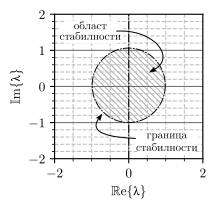
\includegraphics[scale=1]{fig/stab_edit.pdf}
    \caption{Илустрација области и границе стабилности}
    \label{fig:\ID.stab}
\end{figure}

(a) Корени карактеристичниг полинома су $\uplambda_1 = -1$ (двоструки) и $\uplambda_2 = -2$. Пошто се оба корена 
налазе у области стабилности, дати систем је асимптотски стабилан. 

(б) Корени карактеристичног полинома су $\uplambda_{12} = \pm \jj 2$. Пошто постоји једноструки пар 
комплексно конјугованих коренова на граници стабилности систем је гранично стабилан. 

(в) Корени карактреристичног полиома су $\uplambda_{12} = \pm \jj 3$ (двоструки пар). Пошто постоје двоструки корени 
на граници стабилности, дати систем је асимптотски нестабилан.

(г) Корени карактеристичног полинома налазе се решавањем квадратне једначине 
$\uplambda_{12} = 2 \pm \jj$. Пошто се пар коренова налази ван области стабилности систем је асимптотски нестабилан. 

